\section{Thông tin tổng quát về các biến của bộ dữ liệu}

$\indent$
Sau khi làm sạch dữ liệu, ta thực hiện thống kê mô tả cho các biến đã chọn

\begin{minted}{r}
mean<-apply(GPU_new[,numerical],2,mean)
sd<-apply(GPU_new[,numerical],2,sd)
min<-apply(GPU_new[,numerical],2,min)
max<-apply(GPU_new[,numerical],2,max)
median<-apply(GPU_new[,numerical],2,median)
data.frame(mean,sd,min,max,median)
\end{minted}

\begin{figure}[!h]
    \centering
    \fbox{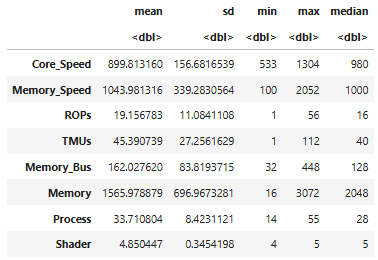
\includegraphics[width=1\linewidth]{images/Screenshot 2026-05-03 043742.png}}
\end{figure}

Tương tự, ta cũng lập bảng tính các giá trị thống kê mô tả cho các biến định lượng trong GPU\_new\_log
\begin{minted}{r}
mean<-apply(GPU_new_log[,numerical],2,mean)
sd<-apply(GPU_new_log[,numerical],2,sd)
min<-apply(GPU_new_log[,numerical],2,min)
max<-apply(GPU_new_log[,numerical],2,max)
median<-apply(GPU_new_log[,numerical],2,median)
data.frame(mean,sd,min,max,median)
\end{minted}

\begin{figure}[!h]
    \centering
    \fbox{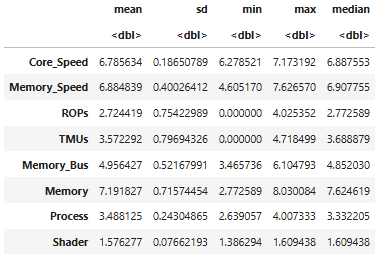
\includegraphics[width=1\linewidth]{images/Screenshot 2026-05-03 043747.png}}
\end{figure}
Để giúp chúng ta hình dung ra bản chất dữ liệu cũng như mối quan hệ giữa chúng dễ dàng hơn khi nhìn vào những con số, ta sẽ biểu diễn lại các dữ liệu này dưới dạng các biểu đồ để dễ quan sát hơn.

\section{Biểu đồ - đồ thị}
$\indent$
Biểu đồ tần suất (histogram) thường dùng để thể hiện phân phối của biến định lượng. Ta vẽ biểu đồ tần suất cho các dữ liệu GPU\_new và GPU\_new\_log. Ta tiến hành vẽ biểu đồ tần suất cho dữ liệu GPU\_new.

\begin{minted}{r}
# Chia layout thành 2 hàng và 4 cột
par(mfrow = c(2, 4), mar = c(4, 4, 2, 1))

# Vẽ histogram cho từng biến numerical trong GPU_new
for (i in 1:length(numerical)) {
 hist_data <- GPU_new[[numerical[i]]]
 hist(hist_data, 
      xlab = names(GPU_new)[which(names(GPU_new) == numerical[i])], 
      main = paste("Histogram of", names(GPU_new)[which(names(GPU_new) == numerical[i])]), 
      labels = TRUE, 
       col = "blue")
}
\end{minted}

\begin{figure}[!h]
    \centering
    \fbox{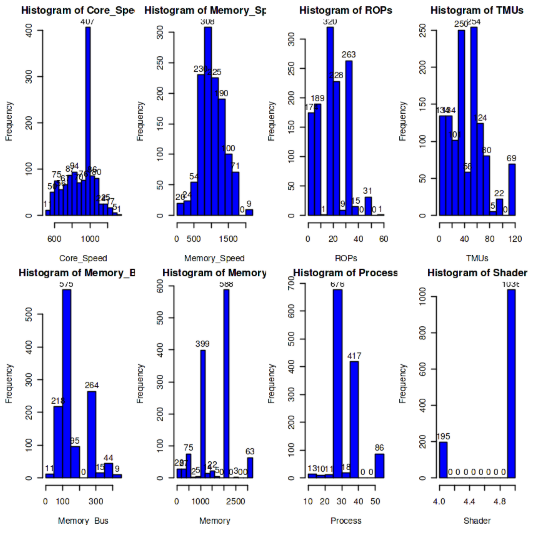
\includegraphics[width=0.8\linewidth]{images/Screenshot 2026-05-03 044605.png}}
\end{figure}

\textbf{Nhận xét:} Ta thấy các biến Process, Memory, TMUs và ROPs có phân phối lệch phải. Biến Core\_Speed có phân phối gần giống phân phối chuẩn. Trong khi đó biến Memory\_Speed có hầu hết các cột cao gần bằng nhau ngoại trừ các cột ở biên, còn biến Memory\_Bus và Shader thì gần như chỉ có một cột, các cột còn lại không đáng kể.

\vspace{0.5em}

Ta tiếp tục tiến hành vẽ biểu đồ tần suất cho dữ liệu của GPU\_new\_log.

\begin{minted}{r}
# Chia layout thành 2 hàng và 4 cột
par(mfrow = c(2, 4), mar = c(4, 4, 2, 1))

# Vẽ histogram cho từng biến numerical trong GPU_new_log
for (i in 1:length(numerical)) {
 hist_data <- GPU_new_log[[numerical[i]]]
 hist(hist_data, 
   xlab = names(GPU_new_log)[which(names(GPU_new_log) == numerical[i])], 
   main = paste("Histogram of log(", names(GPU_new_log)[which(names(GPU_new_log) == numerical[i])], ")"), 
   labels = TRUE, 
   col = "red")
}
\end{minted}

\begin{figure}[!h]
    \centering
    \fbox{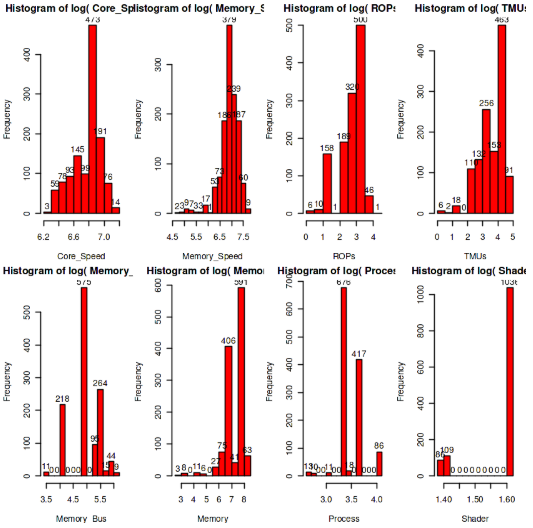
\includegraphics[width=0.8\linewidth]{images/Screenshot 2026-05-03 044612.png}}
\end{figure}

\textbf{Nhận xét:} Ta thấy sau khi chuyển đổi các biến x sang dạng log(x) thì phân phối các biến trở nên gần giống với phân phối chuẩn hơn, ví dụ như biến Memory\_Bus hay Memory\_Speed. Các biến Core\_Speed, Memory, TMUs và ROPs cũng không còn phân phối lệch như trước.

\vspace{0.5em}

Biểu đồ cột (Barplot) thường được dùng để thể hiện phân phối giữa các biến định tính. Ta tiến hành vẽ biểu đồ cột như sau:

\begin{minted}{r}
# Chia layout thành 1 hàng và 3 cột
par(mfrow = c(1, 3), mar = c(4, 4, 2, 1))

# Vẽ bảng barplot thể hiện phân phối biến định luọng
barplot(table(GPU_new$Manufacturer), xlab="Manufacturer", ylab="Frequency", main="Barplot of Manufacturer", col=c("red","green","blue"))
barplot(table(GPU_new$Memory_Type), xlab="Memory_Type", ylab="Frequency", main="Barplot of Memory_Type", col=c("red","green","blue"))
barplot(table(GPU_new$Resolution_WxH), xlab="Resolution_WxH", ylab="Frequency", main="Barplot of Resolution_WxH", col=c("red","green","blue"))
\end{minted}

\begin{figure}[!h]
    \centering
    \fbox{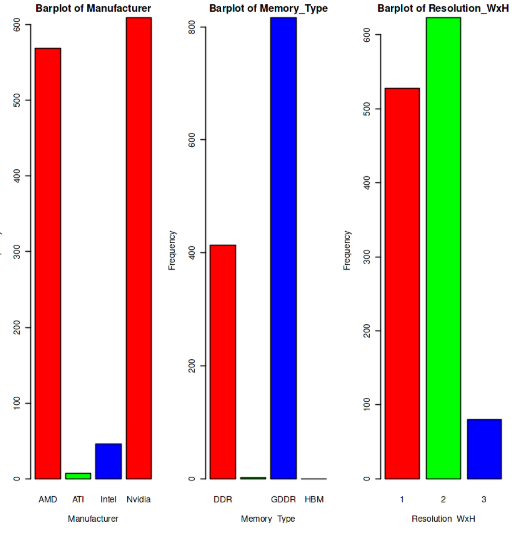
\includegraphics[width=0.8\linewidth]{images/Screenshot 2026-05-03 044739.png}}
\end{figure}

\textbf{Nhận xét:} Ta thấy hầu hết GPU đều được sản xuất bởi AMD và Nvidia, 2 nhà sản xuất còn lại (ATI và Intel) không đáng kể. Chỉ có 2 kiểu bộ nhớ là DDR và GDDR, và đa số thuộc về GDDR. Về chỉ số Resolution\_WxH thì ta thấy không có sự chênh lệch đáng kể giữa 3 cột như 2 biến kia.

\vspace{0.5em}

Biểu đồ boxplot là biểu đồ diễn tả 5 vị trí phân bố của dữ liệu: giá trị nhỏ nhất (min), tứ phân vị thứ nhất (Q1), trung vị (median), tứ phân vị thứ 3 (Q3) và giá trị lớn nhất (max). Ta vẽ biểu đồ boxplot thể hiện phân phối của biến Pixel\_Rate và log(Pixel\_Rate) theo từng phân loại của các biến rời rạc.

\begin{minted}{r}
par(mfrow=c(1,2))
boxplot(Pixel_Rate~Manufacturer, data=GPU_new, main="boxplot of Pixel_Rate for Manufacturer", col="blue")
boxplot(Pixel_Rate~Manufacturer, data=GPU_new_log, main="boxplot of log(Pixel_Rate) for Manufacturer", col="red")
\end{minted}

\begin{figure}[!h]
    \centering
    \fbox{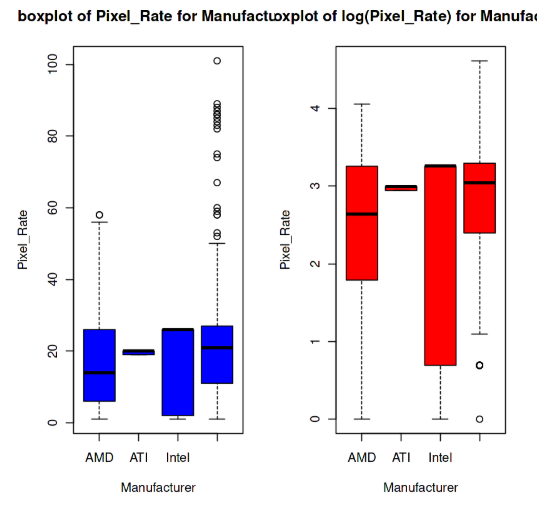
\includegraphics[width=0.6\linewidth]{images/Screenshot 2026-05-03 045147.png}}
\end{figure}

\textbf{Nhận xét:} Ta thấy với nhà sản xuất là AMD và Nvidia thì dung lượng bộ nhớ có phân phối hơi lệch phải, còn với ATI thì lệch trái. Nhưng sau khi lấy log(Pixel\_Rate) thì cả 4 phân phối đều trở thành phân phối chuẩn.

\begin{minted}{r}
par(mfrow=c(1,2))
boxplot(Pixel_Rate~Memory_Type, data=GPU_new, main="boxplot of Pixel_Rate for Memory_Type", col="blue")
boxplot(Pixel_Rate~Memory_Type, data=GPU_new_log, main="boxplot of log(Pixel_Rate) for Memory_Type", col="red")
\end{minted}

\begin{figure}[!h]
    \centering
    \fbox{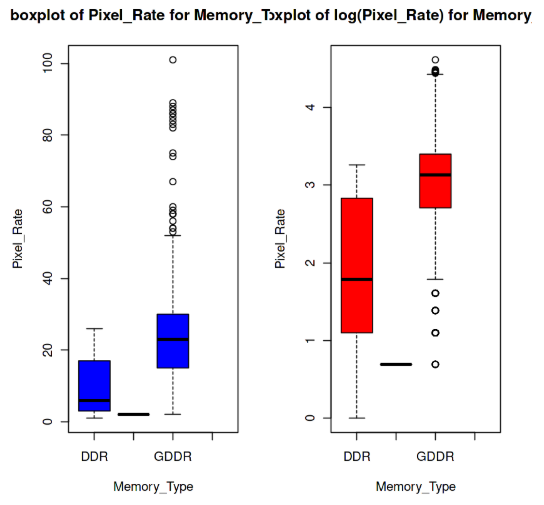
\includegraphics[width=0.6\linewidth]{images/Screenshot 2026-05-03 045152.png}}
\end{figure}

\textbf{Nhận xét:} Với kiểu bộ nhớ GDDR thì dữ liệu hơi lệch phải, còn eDRAM thì hoàn toàn lệch phải. Sau khi lấy log thì phân phối của GDDR đã trở nên phân phối chuẩn, nhưng với eDRAM thì vẫn còn bị lệch.

\begin{minted}{r}
par(mfrow=c(1,2))
boxplot(Pixel_Rate~Resolution_WxH, data=GPU_new, main="boxplot of Pixel_Rate for Resolution_WxH", col="blue")
boxplot(Pixel_Rate~Resolution_WxH, data=GPU_new_log, main="boxplot of log(Pixel_Rate) for Resolution_WxH", col="red")
\end{minted}

\begin{figure}[!h]
    \centering
    \fbox{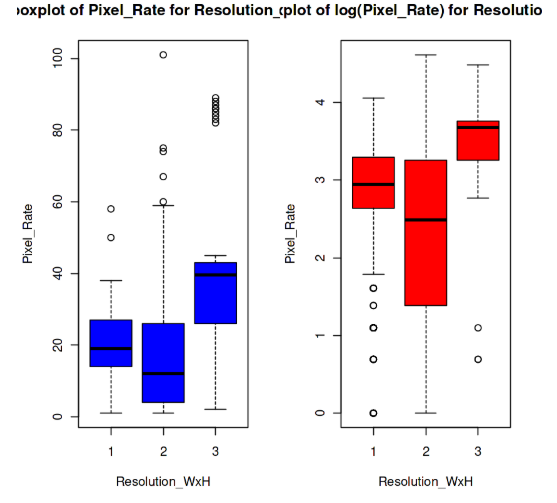
\includegraphics[width=0.6\linewidth]{images/Screenshot 2026-05-03 045158.png}}
\end{figure}

\textbf{Nhận xét:} Các phân phối ở 2 hình trên đều gần với phân phối chuẩn kể cả trước và sau khi dùng hàm log(x).

\vspace{0.5em}

Biểu đồ phân tán là biểu đồ thường được dùng để thể hiện mối liên hệ giữa 2 biến định lượng. Ta vẽ biểu đồ phân tán giữa biến Pixel\_Rate với một số biến định lượng khác.


\begin{minted}{r}
# Chia layout thành 3 hàng và 2 cột
par(mfrow = c(3, 2), mar = c(4, 4, 2, 1))
# Vẽ scatter plot
# Core_Speed vs Pixel_Rate
plot(GPU_new$Core_Speed, GPU_new$Pixel_Rate,
     xlab = "Core_Speed", ylab = "Pixel_Rate",
     main = "Pixel_Rate and Core_Speed", col = "blue", pch = 20)
fit1 <- lm(Pixel_Rate ~ Core_Speed, data = GPU_new)
abline(fit1, col = "red")
# log(Core_Speed) vs log(Pixel_Rate)
plot(GPU_new_log$Core_Speed, GPU_new_log$Pixel_Rate, 
     xlab = "log(Core_Speed)", ylab = "log(Pixel_Rate)", 
     main = "log(Pixel_Rate) and log(Core_Speed)", col = "red", pch = 20)
fit2 <- lm(Pixel_Rate ~ Core_Speed, data = GPU_new_log)
abline(fit2, col = "blue")
# ROPs vs Pixel_Rate
plot(GPU_new$ROPs, GPU_new$Pixel_Rate,
     xlab = "ROPs", ylab = "Pixel_Rate",
     main = "Pixel_Rate and ROPs", col = "blue", pch = 20)
fit3 <- lm(Pixel_Rate ~ ROPs, data = GPU_new)
abline(fit3, col = "red")
# log(ROPs) vs log(Pixel_Rate)
plot(GPU_new_log$ROPs, GPU_new_log$Pixel_Rate, 
     xlab = "log(ROPs)", ylab = "log(Pixel_Rate)", 
     main = "log(Pixel_Rate) and log(ROPs)", col = "red", pch = 20)
fit4 <- lm(Pixel_Rate ~ ROPs, data = GPU_new_log)
abline(fit4, col = "blue")
# Shader vs Pixel_Rate
plot(GPU_new$Shader, GPU_new$Pixel_Rate,
     xlab = "Shader", ylab = "Pixel_Rate",
     main = "Pixel_Rate and Shader", col = "blue", pch = 20)
fit5 <- lm(Pixel_Rate ~ Shader, data = GPU_new)
abline(fit5, col = "red")
# log(Core_Speed) vs log(Pixel_Rate)
plot(GPU_new_log$Core_Speed, GPU_new_log$Pixel_Rate, 
     xlab = "log(Shader)", ylab = "log(Pixel_Rate)", 
     main = "log(Pixel_Rate) and log(Shader)", col = "red", pch = 20)
fit6 <- lm(Pixel_Rate ~ Shader, data = GPU_new_log)
abline(fit6, col = "blue")
# Reset layout
par(mfrow = c(1, 1))
\end{minted}

\begin{figure}[!h]
    \centering
    \fbox{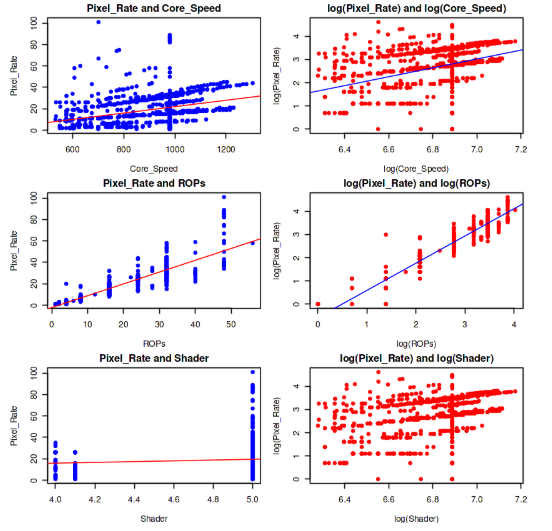
\includegraphics[width=1\linewidth]{images/Screenshot 2026-05-03 050037.png}}
\end{figure}

\textbf{Nhận xét:} Ta thấy biến Pixel\_Rate có quan hệ tuyến tính tăng với biến Core\_Speed. Điều này còn thể hiện rõ hơn giữa biến Pixel\_Rate với ROPs. Và gần như không có mối liên hệ nào giữa Pixel\_Rate và Shader.